\documentclass{standalone}
\usepackage{tikz}
\usetikzlibrary{3d,arrows, calc, backgrounds, petri, positioning, shadows, shapes}


\tikzset{
	persp/.style={scale=3.0,x={(-0.8cm,-0.4cm)},y={(0.8cm,-0.4cm)}, z={(0cm,1cm)}},
	points/.style={fill=white,draw=black,thick}
	grid/.style={very thin,gray},
	axis/.style={->,ultra thick},
	cube/.style={thick, fill=black!15,opacity=0.5},
	cube hidden/.style={dashed},
	block/.style={
		rectangle, rounded corners,
		draw=black!80,
		fill=black!10, fill opacity=0.5,
		text=black!90, text opacity=1.0,
    text height=1.5ex,
    text depth=.25ex,
    text width=6em,
    text centered
	}
}

\tikzstyle{class}			=[rectangle, rounded corners, draw=black, fill=blue!40, drop shadow, text centered, anchor=north, text=white,    text width=3cm]
\tikzstyle{module}		=[rectangle, rounded corners, draw=black, fill=red!40, 	drop shadow, text centered, anchor=north, text=white,    text width=3cm]
\tikzstyle{component}	=[rectangle, rounded corners, draw=black, fill=green,   drop shadow, text centered, anchor=north, text=black!90, text width=3cm]
\tikzstyle{single}		=[text height=1.5ex, text depth=0.25ex]
\tikzstyle{double}		=[text height=4.0ex, text depth=2.75ex]
\tikzstyle{triple}		=[text height=6.5ex, text depth=5.25ex]
\tikzstyle{quadru}		=[text height=9.0ex, text depth=7.75ex]
\newcommand*{\rootPath}{../}

\begin{document}
\begin{tikzpicture}[>=stealth',bend angle=45,auto]
	
	\begin{scope}
		\node [block] (object) 				at (-3,0)					{Objet};
		\node	[anchor=center]					at (-3,1.5)				{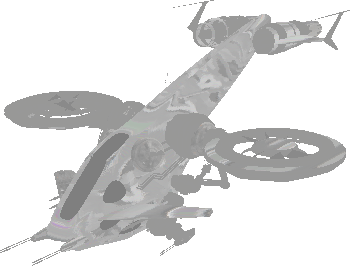
\includegraphics[width=2cm]{\rootPath Imgs/steps/object.png}};
		\node [block] (envmap) 				at (2,0)					{Envmap};
		\node	[anchor=center]					at (2,1.5)				{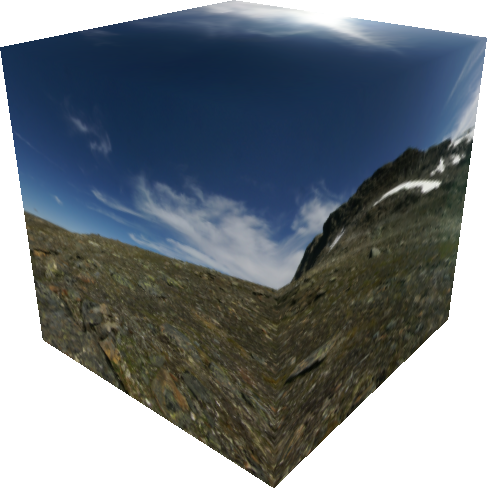
\includegraphics[width=2cm]{\rootPath Imgs/steps/envmap.png}};
  	\node [block] (ambient)				at (-5,-1.2)			{Ambient}
			edge [pre,bend left		= 15] (object);   
		\node [block] (spheres)				at (-1,-1.2)			{Spheres}
			edge [pre,bend right	= 15] (object);      
  	\node [block] (shadow)				at (+1,-2.4)			{Ombre}
			edge [pre,bend right	= 15] (spheres)
			edge [pre,bend left		= 15] (envmap);			
	  \node [block] (rendershadow)	at (+1,-3.6)			{Rendu ombre}
			edge [pre]									(shadow);
  	\node [block] (renderobject)	at (-3,-3.6)			{Rendu objet}
			edge [pre, bend left	= 15]	(ambient)
			edge [pre]									(object)
			edge [pre, bend right	= 15]	(shadow)
			edge [pre, bend right = 10]	(envmap);			
		\node	[anchor=center]					at (0,-6.4)			{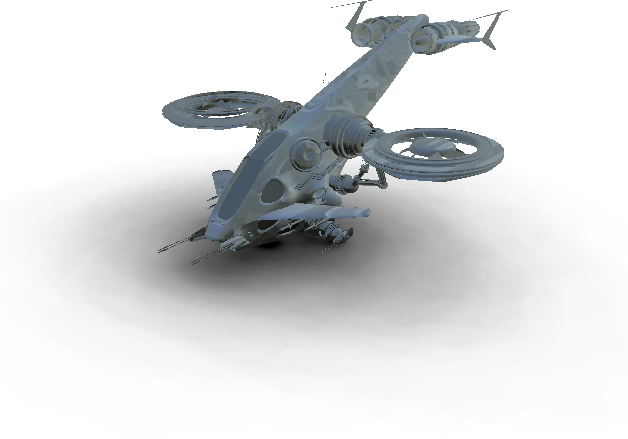
\includegraphics[width=6cm]{\rootPath Imgs/steps/rendered.png}};		
	\end{scope}

	\begin{pgfonlayer}{background}
    \filldraw [line width=4mm, join=round, red!25		]	(-6.2,-0.9)  rectangle (6.2, -1.5);
    \filldraw [line width=4mm, join=round, green!25	]	(-6.2,-2.1)  rectangle (6.2, -2.7);
    \filldraw [line width=4mm, join=round, blue!25	]	(-6.2,-3.3)  rectangle (6.2, -3.9);
    \node[text=black!80,	font=\bfseries, anchor=east] at (6.2, -1.2) {Pr{\'e}calcul};
    \node[text=black!80,	font=\bfseries, anchor=east] at (6.2, -2.4) {Calcul temps r{\'e}el};
    \node[text=black!80, 	font=\bfseries, anchor=east] at (6.2, -3.6) {Rendu temps r{\'e}el};
	\end{pgfonlayer}
  
\end{tikzpicture}
\end{document}